% Diapositiva 33, 34 → El mono | Diapositiva 35 → David | Diapositiva 36 → Danilo

%  El mono (frames 33 y 34) — David (frame 35) — Danilo (frame 36) 
%=============================================
% Puntos 4-10: Mapas de calor, curvas de nivel,
% regiones de bajo error, cortes de profundidad.
%=============================================

% -----------------------------------------------
% FRAME 30a: z = -0.50
% -----------------------------------------------
\begin{frame}{Mapa de Calor: Corte en $z = -0.50$ km — Plano Superficial}

    \begin{columns}[T]

        \column{0.55\textwidth}

        \begin{block}{Corte en $z = -0.50$ km}
            \centering
            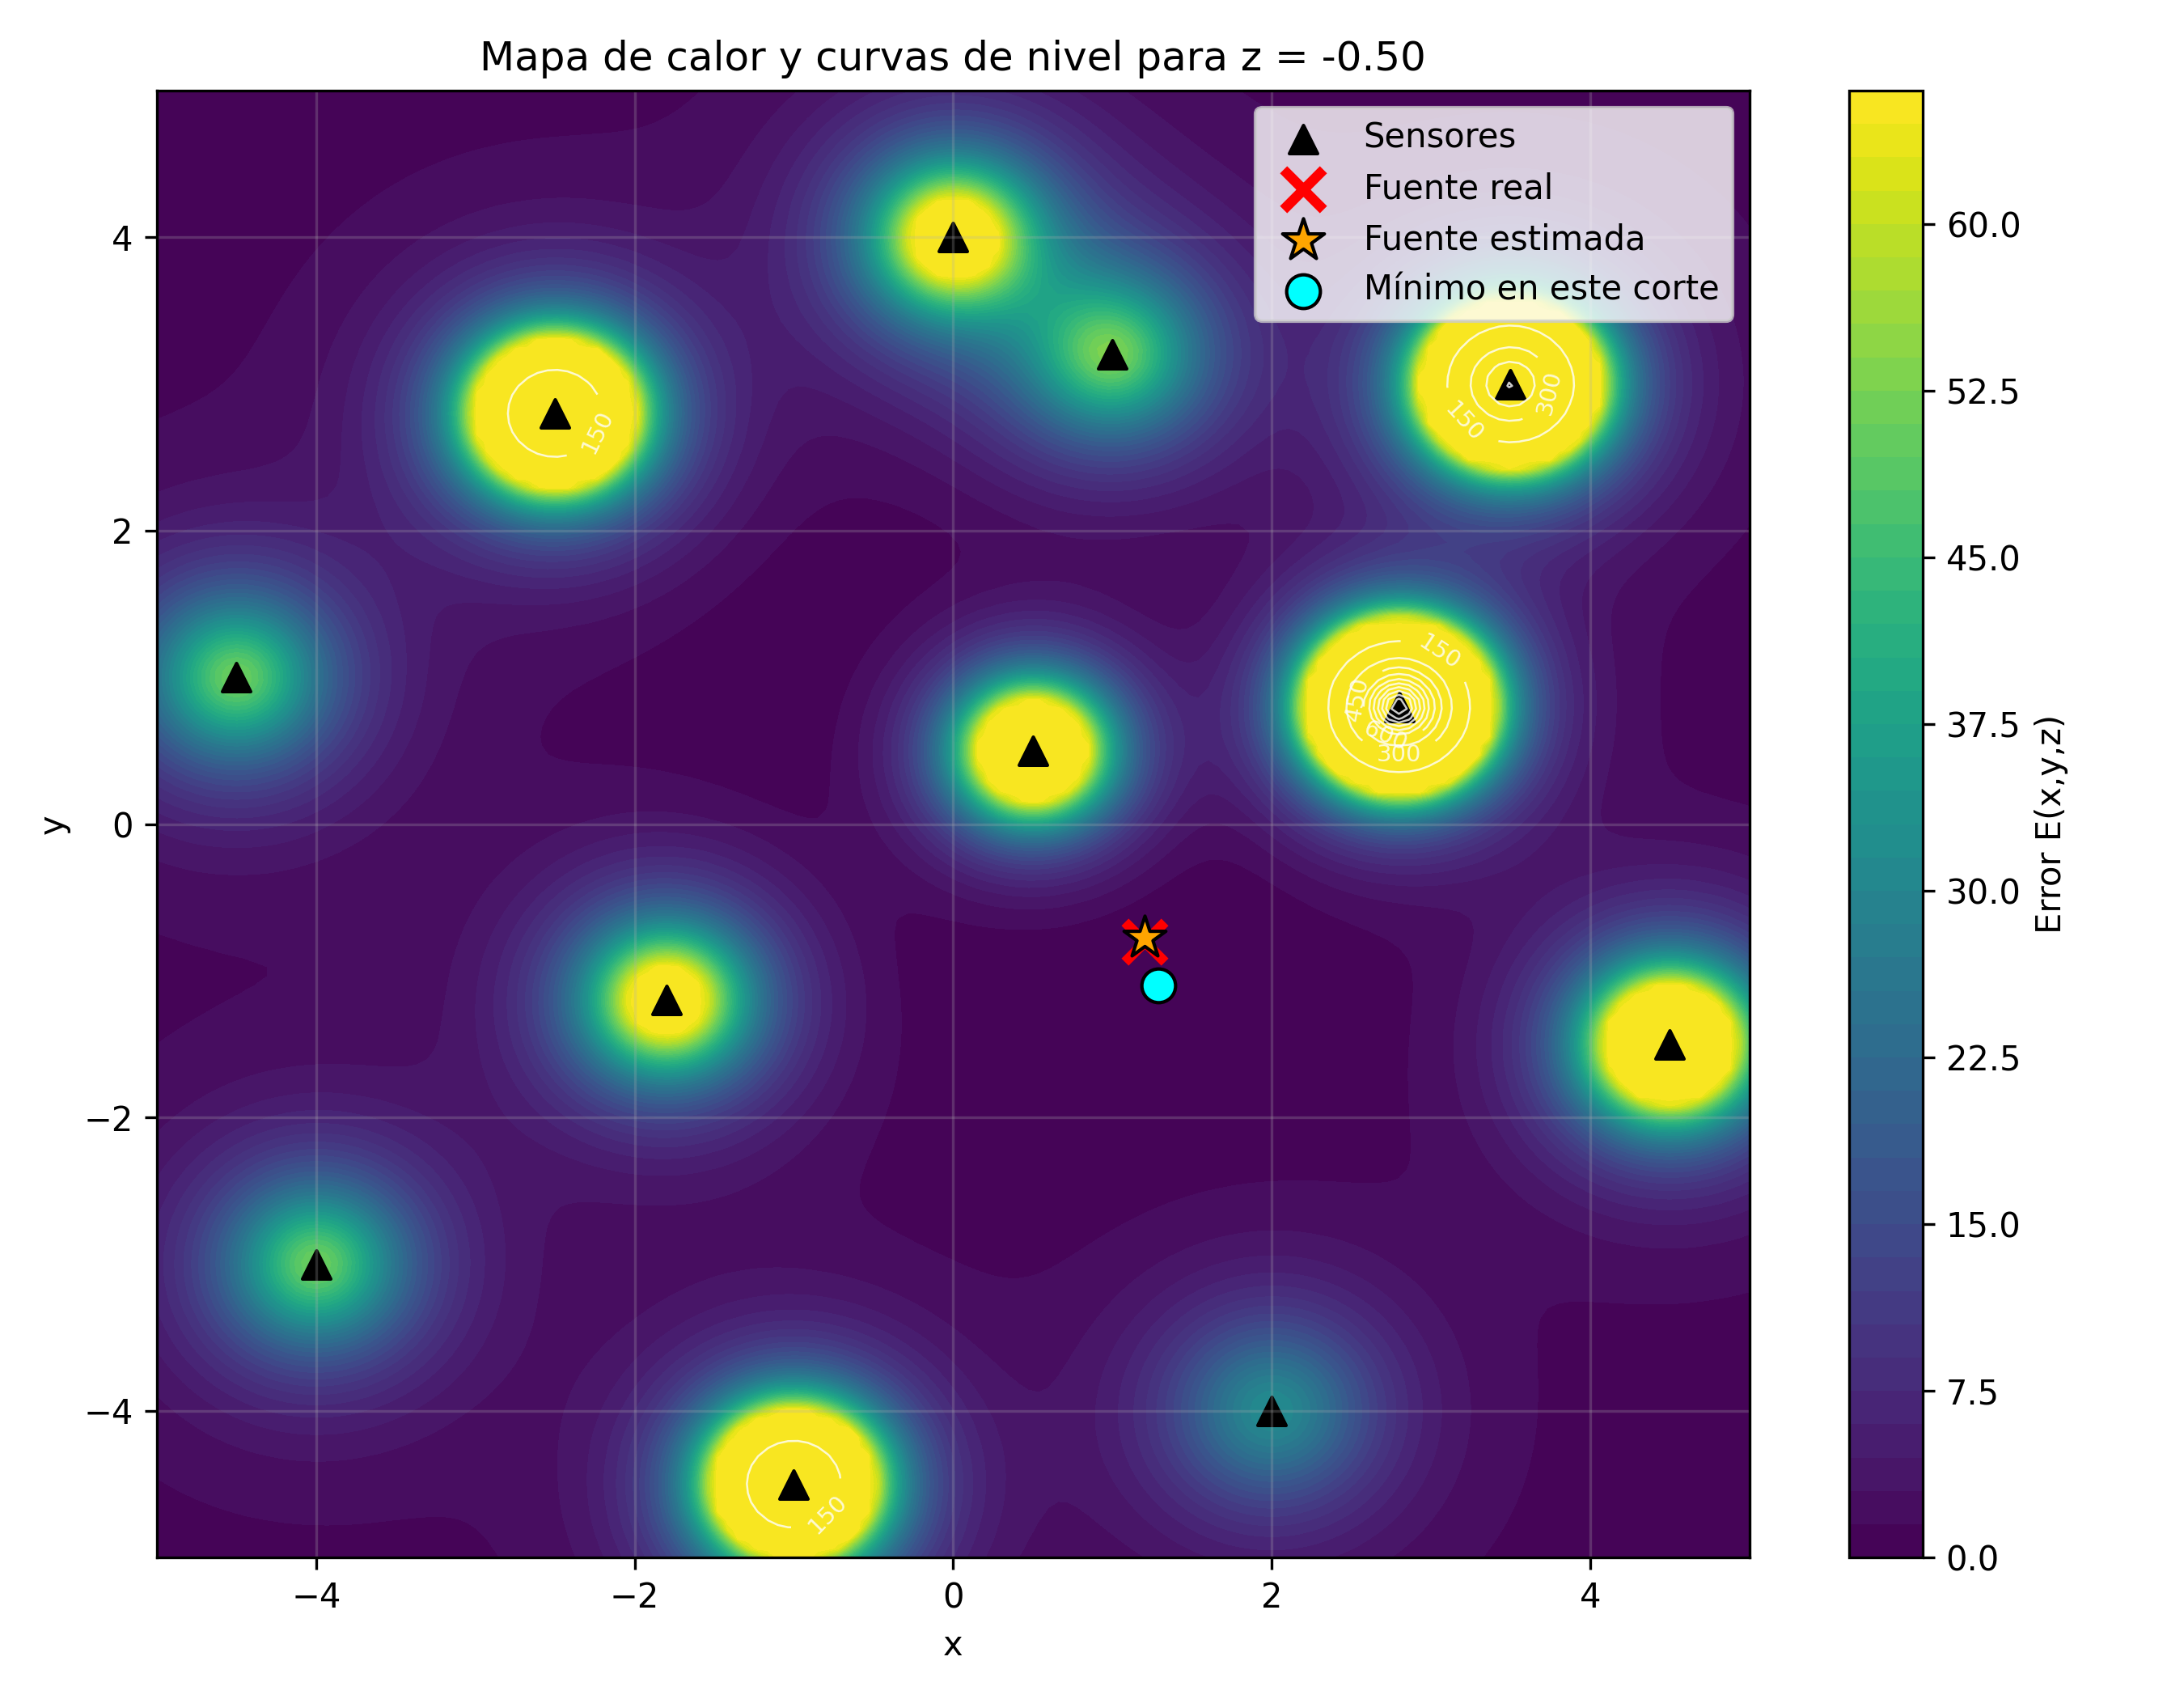
\includegraphics[width=0.95\textwidth]{Imagenes/corte_z_050.png}
        \end{block}

        \column{0.41\textwidth}

        \begin{block}{Interpretación}
            \scriptsize
            \begin{itemize}
                \item Este plano está \textbf{por encima} de la fuente real $z_{\text{real}} = -1.10$ km.
                \vspace{0.1cm}
                \item El error es \textbf{alto y disperso}: no hay una región mínima clara.
                \vspace{0.1cm}
                \item Las curvas de nivel no convergen a un punto definido.
            \end{itemize}
        \end{block}

        \vspace{0.2cm}

        \begin{exampleblock}{¿Qué nos dice?}
            \scriptsize
            A esta profundidad el modelo \textbf{no logra reproducir} las amplitudes observadas, confirmando que la fuente no está aquí.
        \end{exampleblock}

    \end{columns}

    \vspace{0.1cm}
    \begin{center}
        \footnotesize
        \textbf{Zonas frías = error bajo $\Rightarrow$ candidatos a ubicación de la fuente.}
    \end{center}

\end{frame}

% -----------------------------------------------
% FRAME 30b: z = -1.10
% -----------------------------------------------
\begin{frame}{Mapa de Calor: Corte en $z = -1.10$ km — Profundidad Real}

    \begin{columns}[T]

        \column{0.55\textwidth}

        \begin{block}{Corte en $z_{\text{real}} = -1.10$ km}
            \centering
            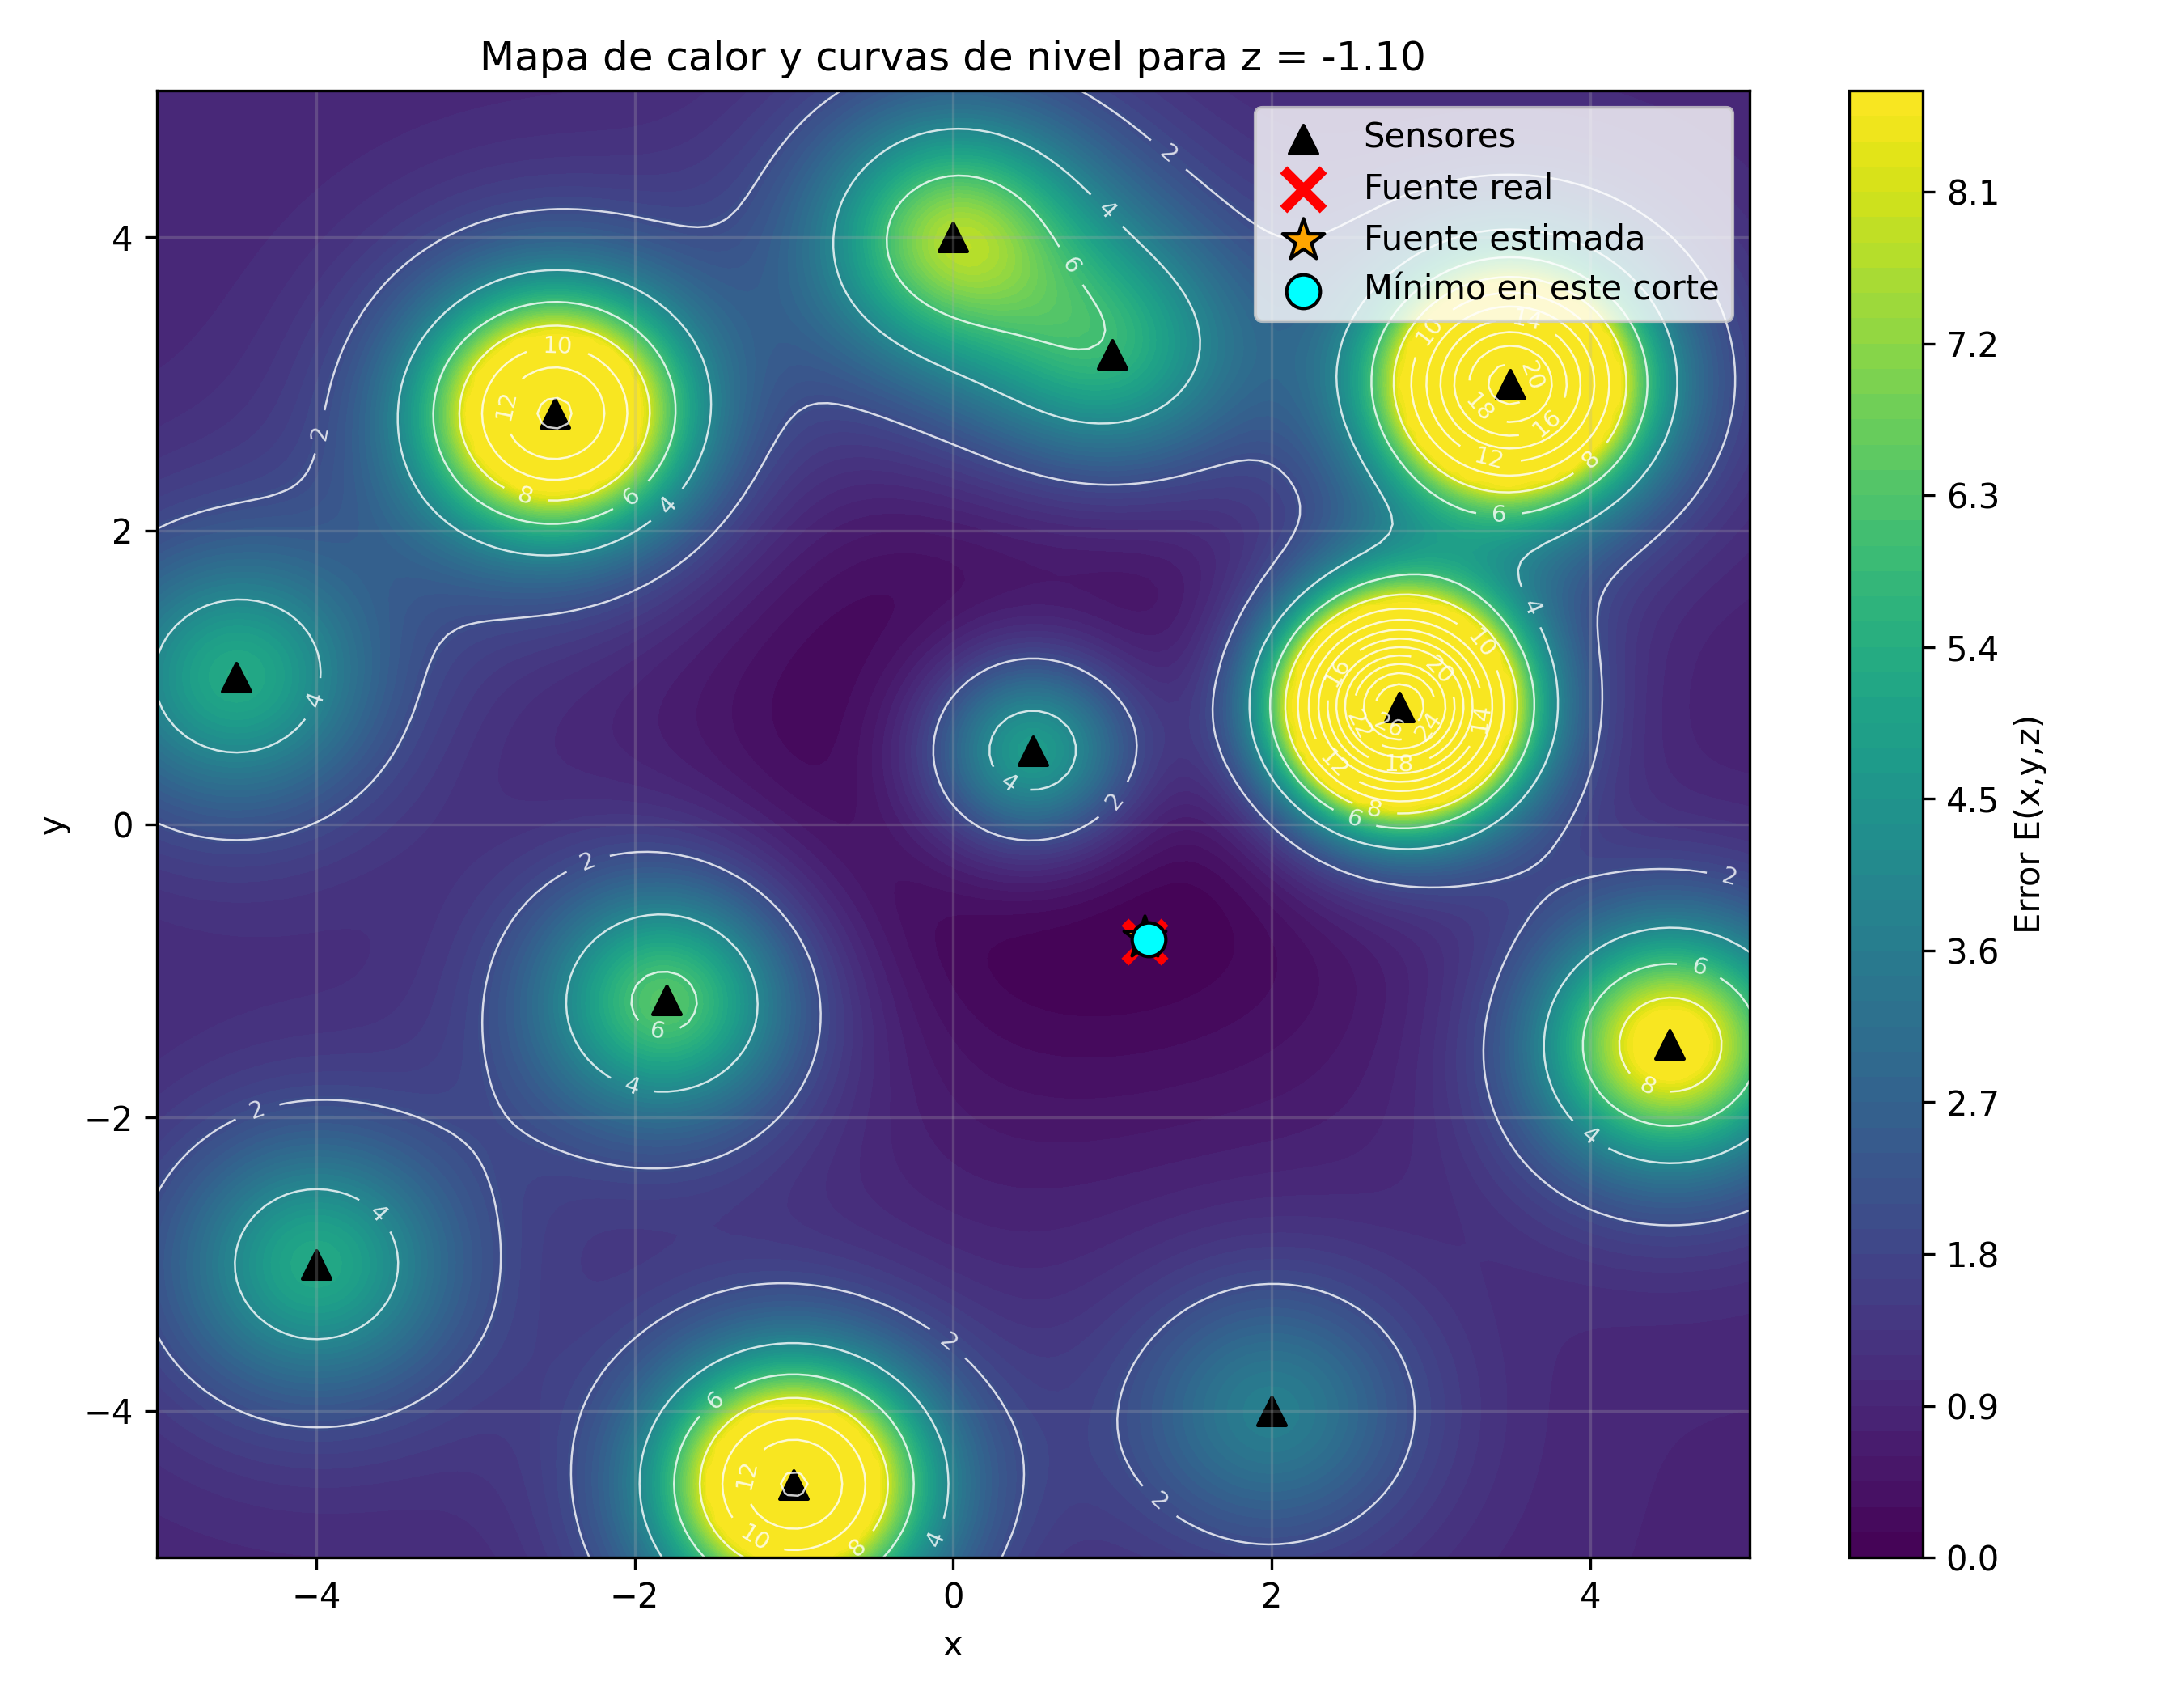
\includegraphics[width=0.95\textwidth]{Imagenes/corte_z_110.png}
        \end{block}

        \column{0.41\textwidth}

        \begin{block}{Interpretación}
            \scriptsize
            \begin{itemize}
                \item Corresponde exactamente a la \textbf{profundidad real} de la fuente simulada.
                \vspace{0.1cm}
                \item La región mínima se \textbf{concentra} claramente alrededor de $(x_{\text{real}},\ y_{\text{real}}) = (1.2,\ -0.8)$ km.
                \vspace{0.1cm}
                \item Las curvas de nivel forman anillos cerrados alrededor del mínimo.
            \end{itemize}
        \end{block}

        \vspace{0.2cm}

        \begin{exampleblock}{¿Qué nos dice?}
            \scriptsize
            El mínimo visual coincide con la \textbf{fuente real simulada}, validando que el modelo captura correctamente la señal sísmica.
        \end{exampleblock}

    \end{columns}

    \vspace{0.1cm}
    \begin{center}
        \footnotesize
        \textbf{Este es el corte más importante: el modelo reproduce mejor las observaciones aquí.}
    \end{center}

\end{frame}

% -----------------------------------------------
% FRAME 30c: z = -1.14  |  Diapositiva 35 → David
% -----------------------------------------------
% David
\begin{frame}{Mapa de Calor: Corte en $z = -1.14$ km — Corte Intermedio}

    \begin{columns}[T]

        \column{0.55\textwidth}

        \begin{block}{Corte en $z = -1.14$ km}
            \centering
            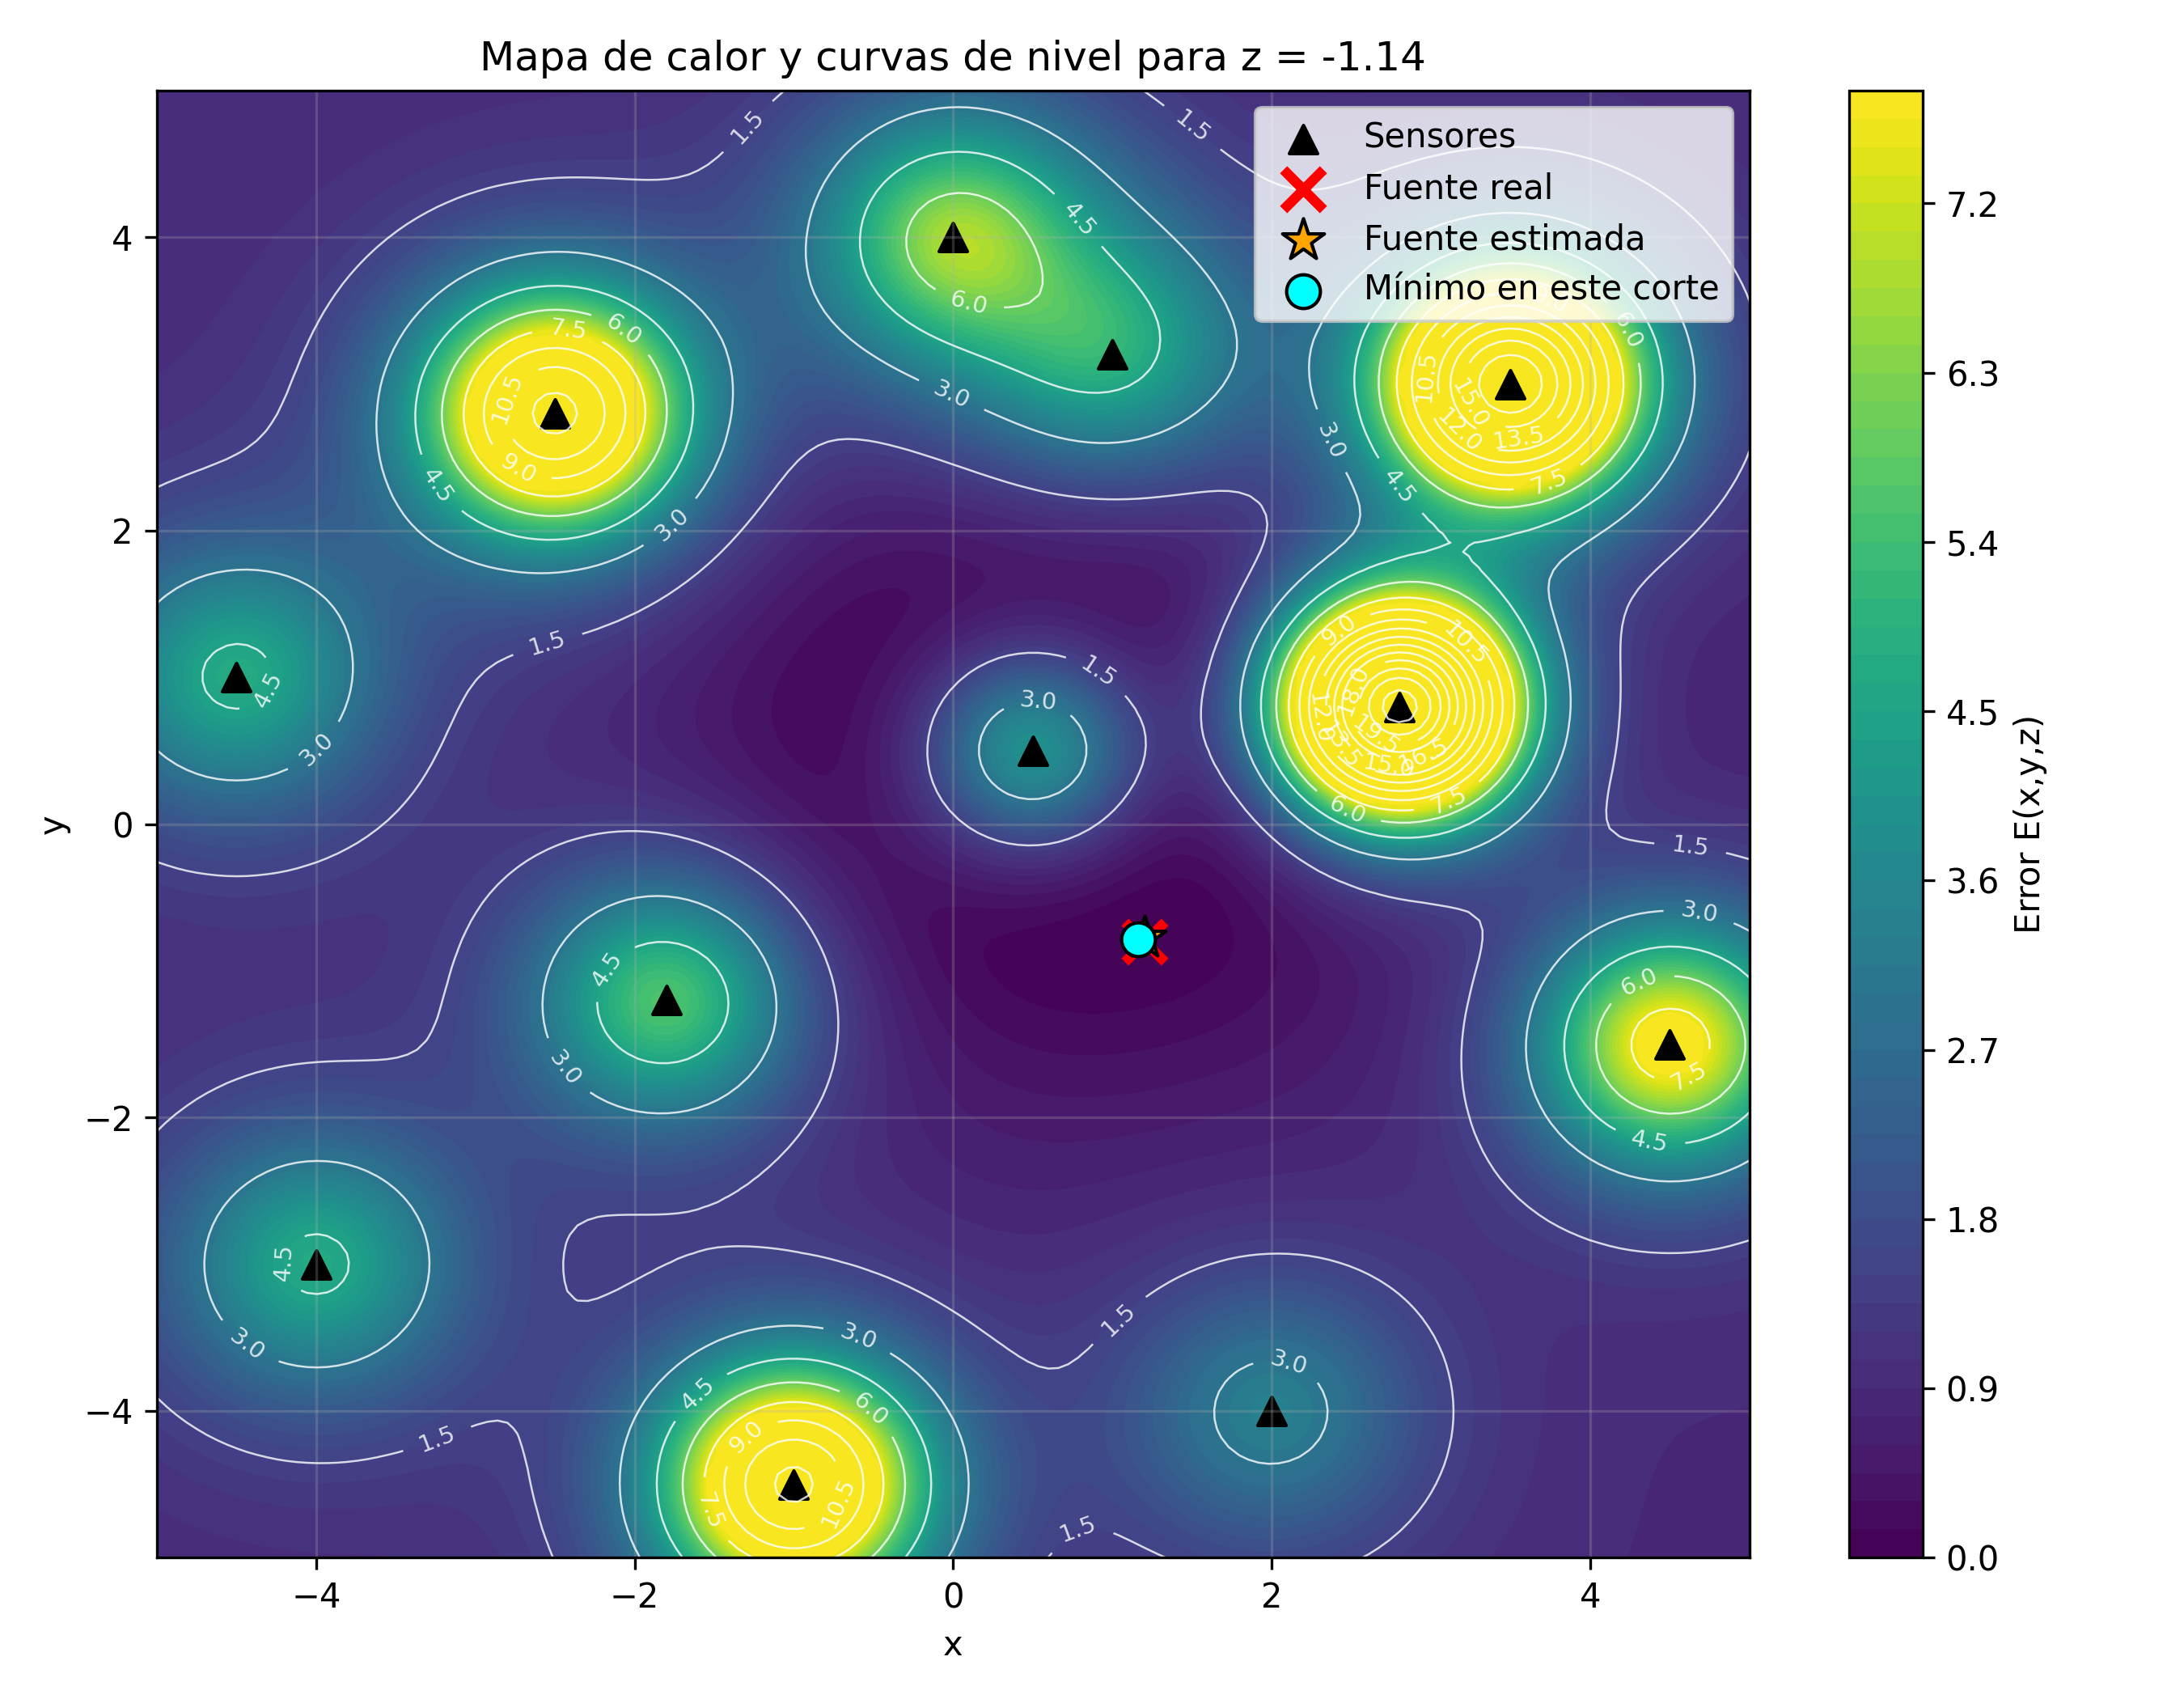
\includegraphics[width=0.95\textwidth]{Imagenes/corte_z_114.png}
        \end{block}

        \column{0.41\textwidth}

        \begin{block}{Interpretación}
            \scriptsize
            \begin{itemize}
                \item Corte \textbf{intermedio} entre $z_{\text{real}} = -1.10$ km y $z_{opt} = -1.22$ km.
                \vspace{0.1cm}
                \item La región mínima sigue \textbf{bien definida} y cercana a la fuente real.
                \vspace{0.1cm}
                \item Confirma la \textbf{estabilidad} del modelo ante pequeñas variaciones de $z$.
            \end{itemize}
        \end{block}

        \vspace{0.2cm}

        \begin{exampleblock}{¿Qué nos dice?}
            \scriptsize
            La región de bajo error se mantiene cerca de $(x_{\text{real}}, y_{\text{real}})$, confirmando la robustez de la solución de Gauss-Newton.
        \end{exampleblock}

    \end{columns}

    \vspace{0.1cm}
    \begin{center}
        \footnotesize
        \textbf{Pequeñas variaciones en $z$ desplazan levemente el mínimo pero no lo destruyen.}
    \end{center}

\end{frame}

% -----------------------------------------------
% FRAME 30d: z = -1.70  |  Diapositiva 36 → Danilo
% -----------------------------------------------
% Danilo
\begin{frame}{Mapa de Calor: Corte en $z = -1.70$ km — Plano Profundo}

    \begin{columns}[T]

        \column{0.55\textwidth}

        \begin{block}{Corte en $z = -1.70$ km}
            \centering
            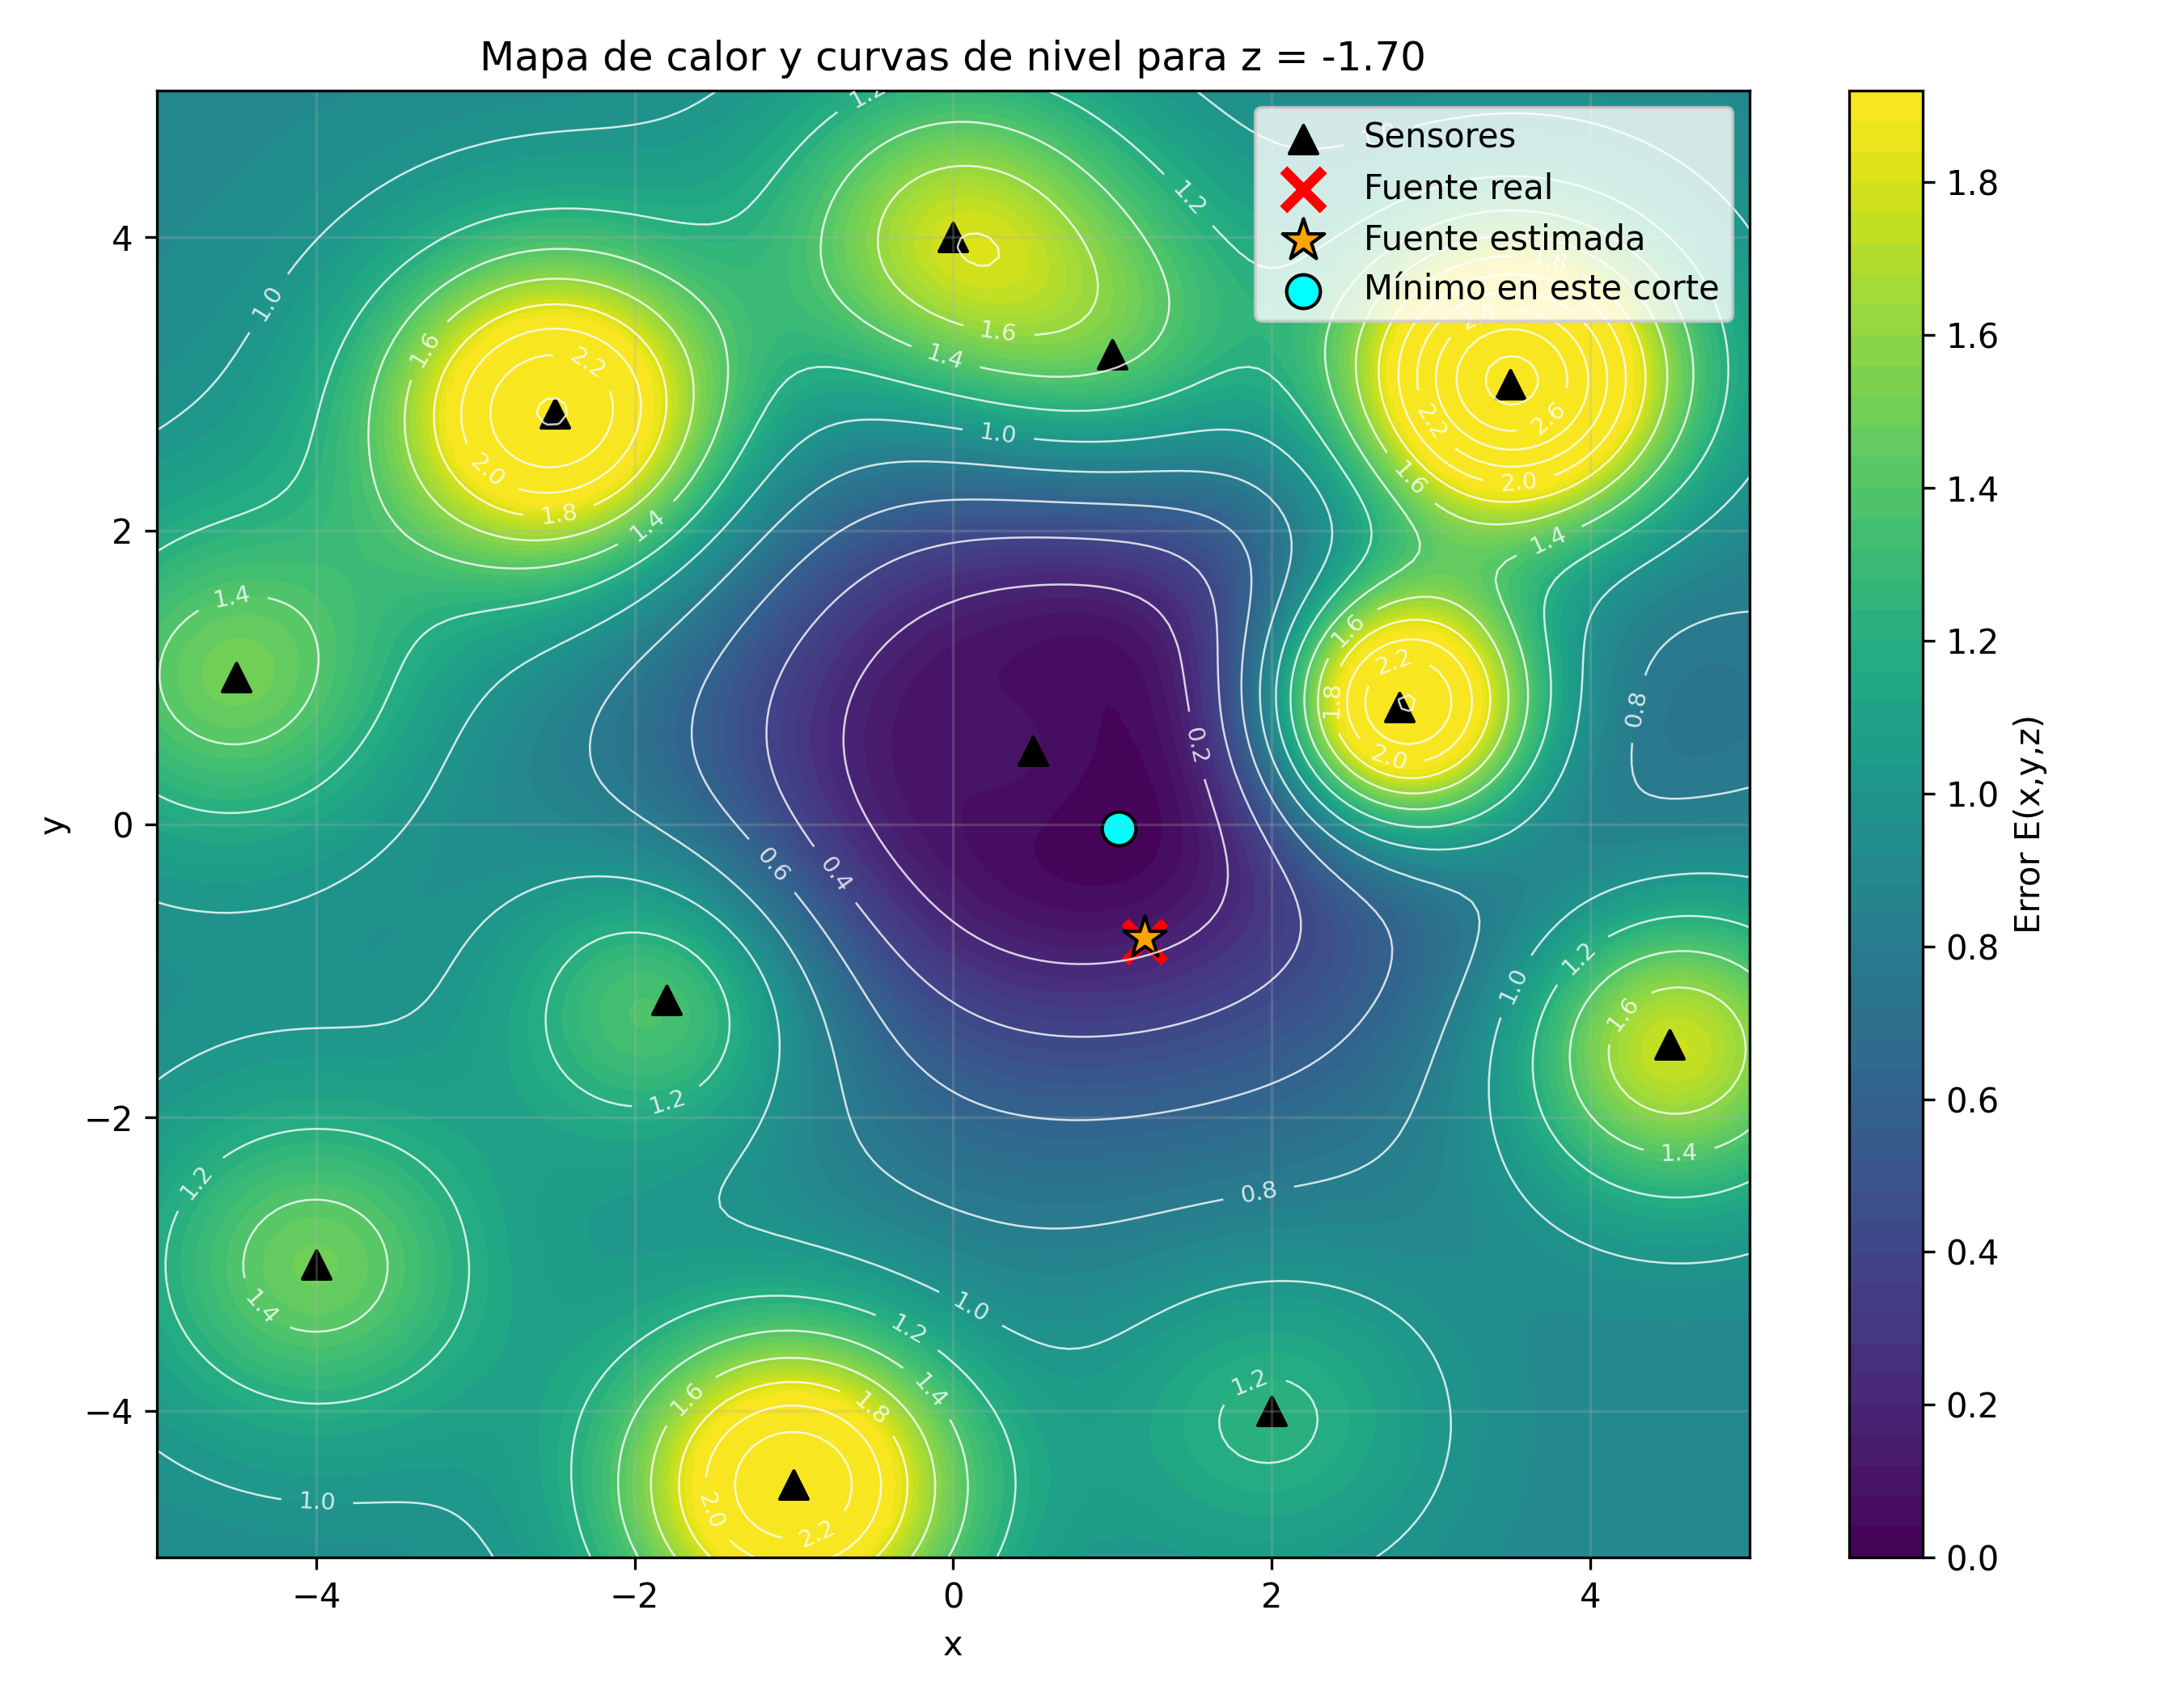
\includegraphics[width=0.95\textwidth]{Imagenes/corte_z_170.png}
        \end{block}

        \column{0.41\textwidth}

        \begin{block}{Interpretación}
            \scriptsize
            \begin{itemize}
                \item Este plano está \textbf{por debajo} de $z_{\text{real}}$ y $z_{opt}$.
                \vspace{0.1cm}
                \item La región mínima se \textbf{aleja y dispersa} respecto a los cortes anteriores.
                \vspace{0.1cm}
                \item El error mínimo en este plano es \textbf{mayor} que en $z_{\text{real}} = -1.10$ km.
            \end{itemize}
        \end{block}

        \vspace{0.2cm}

        \begin{exampleblock}{Conclusión Comparativa}
            \scriptsize
            Al alejarnos de la profundidad real, la función de error \textbf{pierde definición}, confirmando que $z_{\text{real}} = -1.10$ km es la profundidad que mejor explica las observaciones.
        \end{exampleblock}

    \end{columns}

    \vspace{0.1cm}
    \begin{center}
        \footnotesize
        \textbf{Comparar los 4 cortes revela la sensibilidad del modelo ante cambios de profundidad.}
    \end{center}

\end{frame}
